
%%%%%%%%%%%%%%%%%%%%%%%%%%%%%%%%%%%%%%%%%%%%

\section{Propriétés}

    \subsection{Mouvement rectiligne uniforme}

Lorsque nous sommes dans une automobile en mouvement rectiligne uniforme, nous ne ressentons pas le mouvement. Nous pouvons avoir l'impression que c'est le paysage qui est en mouvement.

 En revanche, lorsque l'automobile freine (mouvement non uniforme) ou prend un virage (mouvement non rectiligne), nous ressentons des {\it accélérations}.

De la même façon, dans un train roulant à vitesse constante sur une voie en ligne droite, les passagers ne ressentent pas le mouvement.

\begin{center}
%%%%%%%%%%%%%%%%%%%%%%%%%%%%%%%%%%%%%%%%%%%%%%%%%%%%%%
%%%%%%%%%%%%%%%%%%%%%%%%%%%%%%%%%%%%%%%%%%%%%%%%%%%%%%%%%%%%%%%%%%%%
\def\scl{1}%scaling factor of the picture


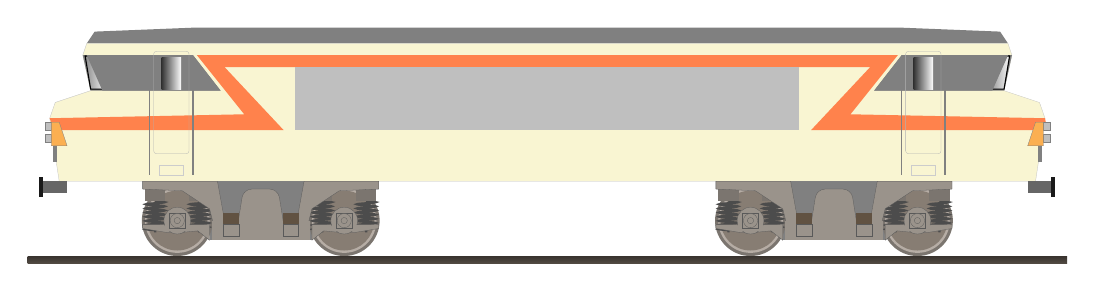
\begin{tikzpicture}[
  scale=\scl,
  beige/.style={color=gray!20!brown!40!yellow!20!},
  orange/.style={color=red!70!yellow!70!},
  wagon/.style={green!70!brown!20!black!75!,draw=black,thick},
 % toit/.style={black!70!brown!20!,draw=gray,thick},!80!gray!10!brown!20!yellow!10!
  %roue/.style={brown!20!black!70!,draw=black,thick},
  fenetre/.style={white,rounded corners = 2pt,draw=black, thick},
  porte/.style={red!55!black,draw=gray!20!, ultra thin},
  porteMotrice/.style={rounded corners = 1pt,draw=gray!60!, ultra thin},
  essieux/.style={gray!20!brown!30!black!50!,draw=gray!70!black, ultra thin},
  grisEssieux/.style={gray!20!brown!30!black!50!}
  ]

  \begin{scope}[xshift=0 cm,yshift=0 cm]%, scale = 0.3
%
%         LIAISONS
%
 % \fill[color=gray,draw=gray!20!, ultra thin] % 
 %(0.15, 0.9) rectangle (12.95, 2.2);

%
%     CORPS DE LA MOTRICE
%

  \fill[color=gray] % 
 (4.5, 2.9) -- (5.75, 2.85) -- (5.85, 2.7) -- (-5.85, 2.7) -- 
 (-5.75, 2.85) -- (-4.5, 2.9) -- cycle;

  \fill[beige,draw=gray!50!, ultra thin] % 
 (5.85, 2.7) -- (5.9, 2.55) -- (5.8, 2.1) -- (6.25, 1.95) -- (6.32, 1.75)
 -- (6.2, 0.95) --  (-6.2, 0.95) -- (-6.32, 1.75) -- (-6.25, 1.95)
 -- (-5.8, 2.1) -- (-5.9, 2.55) -- (-5.85, 2.7) -- cycle;

  \fill[orange] % 
 (4.45, 2.55) -- (3.85, 1.8) -- (6.32, 1.75) -- (6.35, 1.6) -- (3.35, 1.6) -- (4.1, 2.4) 
 -- (-4.1, 2.4) -- (-3.35, 1.6) -- (-6.27, 1.6) -- (-6.32, 1.75) -- (-3.85, 1.8) -- (-4.45, 2.55) -- cycle;

  %  FEUX DROITE
  \fill[color=gray!50!,draw=gray, ultra thin]
 (6.3,1.7) rectangle (6.38, 1.6);
  \fill[color=gray!50!,draw=gray, ultra thin]
 (6.3,1.55) rectangle (6.38, 1.45);
  \fill[color=brown!20!red!50!yellow!70!,draw=gray, ultra thin]
 (6.2,1.7) -- (6.3, 1.7) -- (6.3, 1.4) -- (6.1, 1.4) -- cycle;
  \fill[color=gray]
 (6.23,1.4) rectangle (6.28, 1.2);
  %  FEUX GAUCHE
  \fill[color=gray!50!,draw=gray, ultra thin]
 (-6.3,1.7) rectangle (-6.38, 1.6);
  \fill[color=gray!50!,draw=gray, ultra thin]
 (-6.3,1.55) rectangle (-6.38, 1.45);
  \fill[color=brown!20!red!50!yellow!70!,draw=gray, ultra thin]
 (-6.2,1.7) -- (-6.3, 1.7) -- (-6.3, 1.4) -- (-6.1, 1.4) -- cycle;
  \fill[color=gray]
 (-6.23,1.4) rectangle (-6.28, 1.2);

 % GRILLE
  \fill[color=gray!50!]
 (3.2,1.6) -- (3.2, 2.4) -- 
 (-3.2,2.4) -- (-3.2, 1.6) --  cycle;



\foreach \t in {-1,1}
{
      % PARE BRISE ET GRIS AUTOUR
      % gris
  \fill[color=gray] % 
 (\t*4.5, 2.55) -- (\t*5.9, 2.55) -- (\t*5.8, 2.1) -- (\t*4.15, 2.1) --  cycle;
      % vitre
  \shade[bottom color=gray!5!, top color=gray!90!, shading angle={90}, draw=black]
 (\t*5.8, 2.54) -- (\t*5.87, 2.54) -- (\t*5.8, 2.12) -- (\t*5.6, 2.12) --  cycle;
      % gris
  \fill[color=gray] % 
 (\t*4.5, 2.55) -- (\t*5.85, 2.55) -- (\t*5.65, 2.1) -- (\t*4.15, 2.1) --  cycle;
      % PORTES
    \draw[porteMotrice]
 (\t*4.55, 1.3) rectangle (\t*5, 2.6);
      % MARCHES
    \draw[draw=gray!40!,very thin]
 (\t*4.62, 1.03) rectangle (\t*4.93, 1.15);
      % RAMPES
    \draw[color=gray] (\t*4.5, 1.03) -- (\t*4.5, 2.3);
    \draw[color=gray] (\t*5.05, 1.03) -- (\t*5.05, 2.3);

  % FENÊTRE
  \shade[bottom color=white, top color=black!80!, shading angle={90}]
   (\t*4.65, 2.12) rectangle (\t*4.9, 2.52);
}

 % ESSIEUX 1

\def\y{0.2}
  \foreach \x in {3.64, -3.64}
   {
 \fill[gray] 
  (\x - 0.65, 0.2) rectangle (\x + 0.65, 0.95);
  }



%  ROUES

\def\hauteur{0.45}% de l'axe des roues
\foreach \x in {2.58, 4.7, -4.7, -2.58}
  {
 % gris essieux : gray!20!brown!30!black!50!
    \fill[gray!20!brown!20!black!60!] (\x, \hauteur) circle (0.45 cm);
    \fill[gray!20!brown!40!black!40!] (\x, \hauteur) circle (0.41 cm);
    \fill[gray!10!brown!30!black!60!] (\x, \hauteur) circle (0.38 cm);
    % RESSORT
  \foreach \t in {-1,1}
  {
     \draw[decorate, decoration={snake, segment length=1.5pt, amplitude=1.2mm}, black!70!, thick]
       (\x + \t * 0.28, 0.7) -- (\x + \t * 0.28, 0.3);
    % RESSORT fixation supérieur
     \fill[gray!20!brown!20!black!60!]
       (\x + \t * 0.28 - .13, 0.9) rectangle (\x + \t * 0.28 + .13, 0.7);
  }
  }


 % ESSIEUX 2

\def\y{0.2}
  \foreach \x in {3.64, -3.64}
   {
\foreach \t in {-1,1}
  {  %  montants supérieur
    \coordinate (A) at (\x + \t*1.5, 0.95) ;
    \coordinate (B) at (\x + \t*1.5, 0.85) ;

    \coordinate (C) at (\x + \t*1, 0.83) ;
    \coordinate (D) at (\x + \t*0.65, 0.6) ;

    \coordinate (E) at (\x + \t*0.6, 0.4) ;
    \coordinate (F) at (\x + \t*0.45, 0.4) ;

    \coordinate (G) at (\x + \t*0.55, 0.95) ;
 \fill[essieux] (A) -- (B) -- (C) -- (D) -- (E) -- (F) -- (G) -- cycle;


    %  montant inférieur
    \coordinate (A) at (\x + \t * 1.5,0.4) ;
    \coordinate (B) at (\x + \t * 1.5,0.35) ;

    \coordinate (C) at (\x + \t * 1.2,0.3) ;
    \coordinate (D) at (\x + \t * 1,0.3) ;

    \coordinate (E) at (\x + \t * 0.80,0.32) ;

    \coordinate (F) at (\x + \t * 0.65,0.2) ;
    \coordinate (G) at (\x + \t * 0.65,0.4) ;
 \fill[essieux] (A) -- (B) -- (C) -- (D) -- (E) -- (F) -- (G) -- cycle;

 \fill[essieux] (\x + \t*1.06, \hauteur) circle (0.17 cm);
 \fill[grisEssieux]
 (\x + \t*1.06 + 0.16, 0.4) rectangle (\x + \t*1.06 + -0.16, 0.32);
 \fill[essieux]
 (\x + \t*1.06 + 0.1, \hauteur + -0.1) rectangle (\x + \t*1.06 + -0.1, \hauteur + 0.1);
    \fill[essieux] (\x + \t*1.06, \hauteur) circle (0.09 cm);
    \fill[essieux] (\x + \t*1.06, \hauteur) circle (0.04 cm);

  }

    %  milieux
  %(\x - 0.65, 0.2) rectangle (\x + 0.65, 0.95);
    \coordinate (A) at (\x-0.22, 0.85) ;
    \coordinate (B) at (\x + 0.22, 0.85) ;
    \coordinate (C) at (\x + 0.3, 0.35) ;
    \coordinate (D) at (\x - 0.3, 0.35) ;
 \fill[essieux, rounded corners = 3pt] (A) -- (B) -- (C) -- (D) -- cycle;

    %  milieux inférieur 
  %(\x - 0.65, 0.2) rectangle (\x + 0.65, 0.95);
    \coordinate (A) at (\x - 0.62,0.45) ;
    \coordinate (B) at (\x + 0.62,0.45) ;
    \coordinate (C) at (\x + 0.62,0.2) ;
    \coordinate (D) at (\x - 0.62,0.2) ;
 \fill[grisEssieux] (A) -- (B) -- (C) -- (D) -- cycle;

\foreach \t in {-1,1}    % silent bloc
  {
  \fill[brown!30!black!80!]
 (\x + \t * 0.38 - 0.1, 0.55) rectangle (\x + \t * 0.38 + 0.1, 0.35);
  \fill[essieux]
 (\x + \t * 0.38 - 0.1, 0.4) rectangle (\x + \t * 0.38 + 0.1, 0.25);
  }
  }

% BAS DE CAISSE


 % BUTOIR GAUCHE
  \fill[color=gray!80!black] % 
 (-6.1, 0.8) rectangle (-6.4, 0.95);
  \fill[color=black!80!gray] % 
 (-6.4, 0.75) rectangle (-6.45, 1);

 % BUTOIR DROIT
  \fill[color=gray!80!black] % 
 (6.1, 0.8) rectangle (6.4, 0.95);
  \fill[color=black!80!gray] % 
 (6.4, 0.75) rectangle (6.45, 1);

  % RAIL
  \shade[bottom color=brown!20!gray!60!black, top color=brown!20!gray!40!black]
 (6.6, 0) rectangle (-6.6, -0.1);

  \end{scope}
%
%
\end{tikzpicture}
%

\end{center}


  \subsection{Principe de relativité}

Énoncé par galilée au {\footnotesize XVII} $^\text{e}$ siècle, il exprime le fait que les lois de la physique restent les mêmes dans les différents référentiels, en mouvement rectiligne uniforme les uns avec les autres.

    \subsubsection{Exemple}

On observe la chute d'une balle dans le champ de pesanteur. Elle est accélérée vers le bas et son mouvement est rectiligne. Cette trajectoire met en évidence la verticale du lieu ou l'on réalise l'expérience. Cette expérience s'interprète dans le paradigme de la mécanique classique à l'aide de la force gravitationnelle que la Terre exerce sur la balle et par la loi reliant la force au mouvement.

\begin{center}
\input{./relativiteMouvements/mouvement/chuteSimple.tex}
\end{center}

Si l'on reproduit cette expérience dans un train en mouvement rectiligne uniforme, le principe d'inertie nous dit que le mouvement doit être identique, puisque les lois dans ce référentiel doivent être identiques.

\begin{center}
\input{./relativiteMouvements/mouvement/chuteWagon.tex}
\end{center}

  \subsection{Relativité des mouvements}

Le mouvements d'un objet dépend du référentiel dans lequel le mouvement est observé.

    \subsubsection{Additivité des vitesses}

Un train roule à la vitesse de 40 km/h. Un voyageur marche dans le couloir de ce train.
% à la vitesse de 5 km/h


\begin{center}
\input{./relativiteMouvements/mouvement/marcheWagon.tex}
\end{center}

%Un voyageur marche dans le couloir d'un train à la vitesse de 5 km/h. Le train roulant à la vitesse de 100 km/h. 

Pour un observateur dans le référentiel terrestre, le train a une vitesse de 40 km/h et le voyageur a une vitesse de 45 km/h. 

Le voyageur a une vitesse de 5 km/h dans le référentiel du train.

    \subsubsection{Relativité des trajectoires}

Dans le référentiel du train, la chute d'une balle lachée par un voyageur est rectiligne.

Dans le référentiel terrestre, la trajectoire de la balle est une courbe.

% \subsection{}

%%%%%%%%%%%%%%%%%%%%%%%%%%%%%%%%%%%%%%%%%%%{\it }



